\documentclass[nooutcomes]{ximera}
\usepackage{booktabs}
%% handout
%% space
%% newpage
%% numbers
%% nooutcomes

\renewcommand{\outcome}[1]{\marginpar{\null\vspace{2ex}\scriptsize\framebox{\parbox{0.75in}{\begin{raggedright}\textbf{P\arabic{problem} Outcome:} #1\end{raggedright}}}}}

\renewenvironment{freeResponse}{
\ifhandout\setbox0\vbox\bgroup\else
\begin{trivlist}\item[\hskip \labelsep\bfseries Solution:\hspace{2ex}]
\fi}
{\ifhandout\egroup\else
\end{trivlist}
\fi}

\newcommand{\RR}{\mathbb R}
\renewcommand{\d}{\,d}
\newcommand{\dd}[2][]{\frac{d #1}{d #2}}
\renewcommand{\l}{\ell}
\newcommand{\ddx}{\frac{d}{dx}}
\everymath{\displaystyle}
\newcommand{\dfn}{\textbf}
\newcommand{\eval}[1]{\bigg[ #1 \bigg]}


\title{Breakout Session 11 Solutions}  

\begin{document}
\begin{abstract}
  % \textbf{A look back:} In the previous (February 9, 2016) Breakout Session you were introduced to the sum, product, and quotient rules for computing derivatives.
  % These rules help us to compute derivatives quickly and accurately.

  % \textbf{Overview:} In today's (February 11, 2016) Breakout Session you'll practice how to evaluate special trigonometric limits and the basic derivatives of trigonometric functions.

  % \textbf{A look ahead:} In the next (February 16, 2016) Breakout Session you will practice real world interpretations of derivatives (as rates of change) and learn the last major differentiation rule.
\end{abstract}
\maketitle

%\section{Learning Outcomes}
% \label{section:learning-outcomes}
% {\small
% The following outcomes are \emph{not an exhaustive} list of the skills you will need to develop and integrate for demonstration on quizzes and exams.
% This list is meant to be a starting point for conversation (with your Lecturer, Breakout Session Instructor, and fellow learners) for organizing your knowledge and monitoring the development of your skills.

% \subsection*{Learning Outcomes for Derivatives as Rates of Change}
% \begin{itemize}
%   \item
%     Find velocity and acceleration and use them to determine information about position.

%   \item 
%     Determine average and instantaneous growth rates. 

%   \item 
%     Calculate average and marginal costs. 

%   \item 
%     Identify applications of the derivative.

%   \item 
%     Assign meaning to the first and second derivatives of a position function.

%   \item 
%     Interpret the derivative as information about growth. 
% \end{itemize}

% \subsection*{Learning Outcomes for Chain Rule}
% \begin{itemize}
%   \item
%     Take derivatives of compositions of functions using the chain rule using both versions. 

%   \item
%     Recognize a composition of functions.

%   \item 
%     Take derivatives that require repeated use of the Chain Rule.

%   \item
%     Take derivatives that require the use of multiple derivative rules.

%   \item 
%     Use order of operations in situations requiring multiple derivative rules.
% \end{itemize}}

% \newpage

\begin{problem}
  \outcome{Recognize a composition of functions.}
For the following problems, the derivative is given.  Determine which function was the original function.
	\begin{enumerate}[label=\roman*.]
	
		\item  The derivative is $f'(x) = \cos (x) e^{\sin x}$.  Which is the original function?
		
			\begin{enumerate}
			
			\item  $f(x) = (\sin x)(e^x)$
			\item  $f(x) = \sin (e^x)$
			\item  $f(x) = e^{\sin x}$
			\item  $f(x) = e^{x \sin x}$
			
				\begin{freeResponse}
				Since
				$$ \ddx \left( e^{\sin x} \right) = e^{\sin x} \cdot \cos x = \cos(x) e^{\sin x} $$
				the correct answer is (c).  
				\end{freeResponse}
				
			\end{enumerate}
			
			
			
		\item  The derivative is $g'(x) = 4 \left( \tan (x^4 - 5x) \right)^3 \sec^2(x^4-5x)(4x^3-5)$.  Which is the original function?
		
			\begin{enumerate}
			
			\item  $g(x) = \left( \tan x - 5x \right)^4$
			\item  $g(x) = \tan^4x - 5x^4$
			\item  $g(x) = \tan(x^4 - 5x)$
			\item  $g(x) = \tan^4(x^4-5x)$
			
				\begin{freeResponse}
				Since 
				$$\ddx \left( \tan^4(x^4-5x) \right) = 4 \tan^3(x^4-5x) \sec^2(x^4-5x) (4x^3-5)$$ 
				the correct answer is (d).  Notice that $\tan^3(x^4-5x) = \left( \tan(x^4-5x) \right)^3$ are (slightly) different notations for the exact same expression.
				\end{freeResponse}
				
			\end{enumerate}
			
	\end{enumerate}
\end{problem}

\begin{problem}
  \outcome{Take derivatives of compositions of functions using the chain rule}
  \outcome{Recognize a composition of functions.}
  A table of values for $f(x)$ and $f'(x)$ is shown below:

  \begin{center}
    \begin{tabular}{ccc}
      \toprule\\
      $x$ & $f(x)$ & $f'(x)$ \\
      \midrule\\
      1 & 3 & 4\\
      3 & 4 & 5\\
      4 & 6 & 3\\
      \bottomrule
    \end{tabular}
  \end{center}

  Evaluate $\displaystyle\ddx f(f(x))$ at $x = 3$.
  \begin{itemize}
    \item[(a)] 6
    \item[(b)] 25
    \item[(c)] 5
    \item[(d)] 15
    \item[(e)] DNE
    \item[(f)] None of the previous answers.
  \end{itemize}
  \begin{freeResponse}
    The answer is (d):
    \begin{align*}
      \eval{\ddx f(f(x))}_{x = 3} &= f'(f(3)) \cdot f'(3) \\
      &= f'(4)\cdot 5 \\
      &= 3 \cdot 5 = 15
    \end{align*}
  \end{freeResponse}
\end{problem}

\begin{problem}
  \outcome{Take derivatives of compositions of functions using the chain rule.}
  \outcome{Recognize a composition of functions.}
  Given the following graphs of $f(x)$ and $g(x)$ (both piecewise
  linear functions), define new functions $u(x) = f(g(x))$ and
  $v(x) = f(x)g(x)$.  Find:

  \begin{image}
    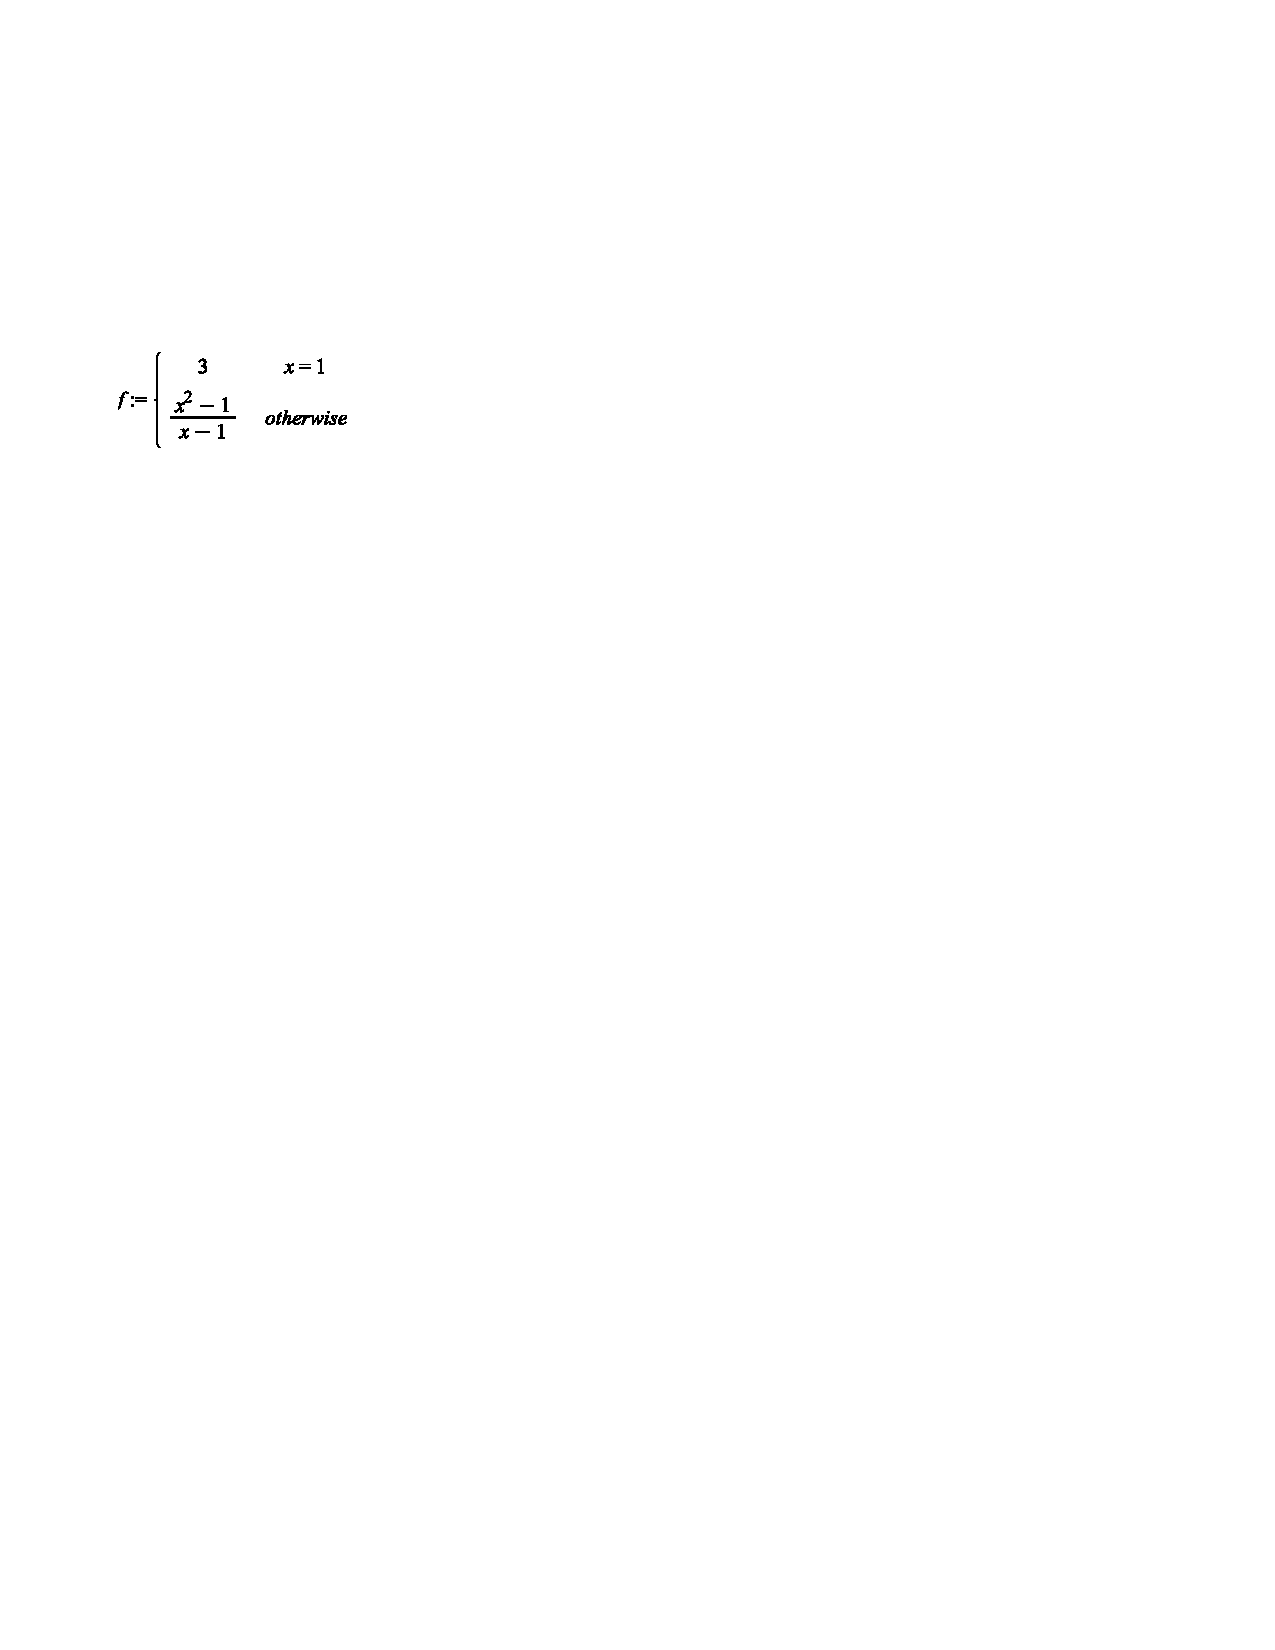
\includegraphics[trim= 170 420 250 230]{Images/Figure7.pdf}
  \end{image}

  \begin{enumerate}
	
  \item $u'(1)$
    \begin{freeResponse}
      $u'(x) = \ddx(f(g(x))) = f'(g(x)) \cdot g'(x)$.  So,
      \begin{align*}
        u'(1) &= f'(g(1)) \cdot g'(1) \\
              &= f'(1) \cdot (-1) \\
              &= (2)(-1) = -2 
      \end{align*}  
    \end{freeResponse}
		
		
		
	
  \item $v'(1)$
    \begin{freeResponse}
      $v'(x) = \ddx(f(x)g(x)) = f'(x)g(x) + f(x)g'(x)$.  So,
      \begin{align*}
        v'(1) &= f'(1) g(1) + f(1) g'(1) \\
              &= (2)(1) + (2)(-1) \\
              &= 0
      \end{align*}
    \end{freeResponse}
  \end{enumerate}
\end{problem}

\begin{problem}
    \outcome{Take derivatives of compositions of functions using the chain rule.}
    \outcome{Recognize a composition of functions.}
Suppose the line tangent to the graph of $f(x)$ at $x=1$ is $y=6x-7$.  Find an equation of the line tangent to the following curves at $x=1$:
	\begin{enumerate}
	
	\item  $g(x) = 5(f(x))^4$  
		\begin{freeResponse}
		First, in the equation of the tangent line to $f(x)$ at $x=1$, when $x=1$ we have that $y= 6(1) - 7 = -1$.  Thus $f(1) = -1$ and therefore $g(1) = 5(-1)^4 = 5$.  Hence, a point on our line is $(1,5)$.  Also, since the slope of this tangent line is $m=6$, we know that $f'(1) = 6$.
		
		Now, by the chain rule we have that $g'(x) = 5 \cdot 4 (f(x))^3 \cdot f'(x)$.  So $g'(1) = 20(f(1))^3 \cdot f'(1) = 20(-1)^3 (6) = -120.$  Thus, the equation of the line tangent to the graph of $y = g(x)$ at $x=1$ is
		$$ y - 5 = -120(x-1) $$
		$$ y = -120x + 125 $$
		\end{freeResponse}

	\item  $h(x) = x^2 (f(x^3))$
		\begin{freeResponse}
		$h(1) = 1^2 \cdot f(1^3) = f(1) = -1$.  By the product and chain rules:
		$$ h'(x) = 2x(f(x^3)) + x^2(f'(x^3) \cdot 3x^2) = 2x(f(x^3)) + 3x^4(f'(x^3)) $$
		Thus, $h'(1) = 2f(1) + 3f'(1) = 2(-1) + 3(6) = -2 + 18 = 16$.  So, the equation of the line tangent to the graph of $y=h(x)$ at $x=1$ is
		$$ y- (-1) = 16(x-1) $$
		$$ y = 16x - 17 $$
		\end{freeResponse}
	\end{enumerate}		
\end{problem}

\begin{problem}
  \outcome{Take derivatives of compositions of functions using the chain rule.}
  \outcome{Recognize a composition of functions.}
Differentiate each function (with respect to $x$)
	\begin{enumerate}
	
	%part a
	\item  $\cos \left( \sqrt{x+7} \right) $
		\begin{freeResponse}
		\begin{align*}
		\ddx \left( \cos \left( \sqrt{x+7} \right) \right) &= -\sin \left( \sqrt{x+7} \right) \cdot \frac{1}{2} (x+7)^{\frac{-1}{2}} (1) \\
		&= \frac{-\sin \left( \sqrt{x+7} \right) }{2 \sqrt{x+7}}
		\end{align*}
		\end{freeResponse}
		
	%part b
	\item  $\sqrt{ \cos x + 7}$
		\begin{freeResponse}
		\begin{align*}
		\ddx \left( \sqrt{ \cos x + 7} \right) &= \frac{1}{2} \left( \cos x + 7 \right)^{\frac{-1}{2}} \left( -\sin x \right) \\
		&= \frac{- \sin x }{2 \sqrt{\cos x + 7 }}
		\end{align*}
		\end{freeResponse}
		
	%part c
	\item $\sqrt{\cos x} + 7$
		\begin{freeResponse}
		\begin{align*}
		\ddx \left( \sqrt{\cos x} + 7 \right) &=  \frac{1}{2} \left( \cos x \right)^{\frac{-1}{2}} \left( -\sin x \right) + 0  \\
		&= \frac{- \sin x}{2 \sqrt{\cos x}}
		\end{align*}
		\end{freeResponse}
		
	%part d
	\item  $\cos \left( \sqrt{x} + 7 \right)$
		\begin{freeResponse}
		\begin{align*}
		\ddx \left( \cos \left( \sqrt{x} + 7 \right) \right) &= - \sin \left( \sqrt{x} + 7 \right) \cdot \frac{1}{2} x^{\frac{-1}{2}} \\
		&=  \frac{- \sin \left( \sqrt{x} + 7 \right) }{2 \sqrt{x}}
		\end{align*}
		\end{freeResponse}
	\end{enumerate}
\end{problem}

\begin{problem}
  \outcome{Assign meaning to the first and second derivatives of a position function.}
  \outcome{Find velocity and acceleration and use them to determine information about position.}
The graph of $s=f(t)$ is the position of an object moving along a number line.
	\begin{image}
	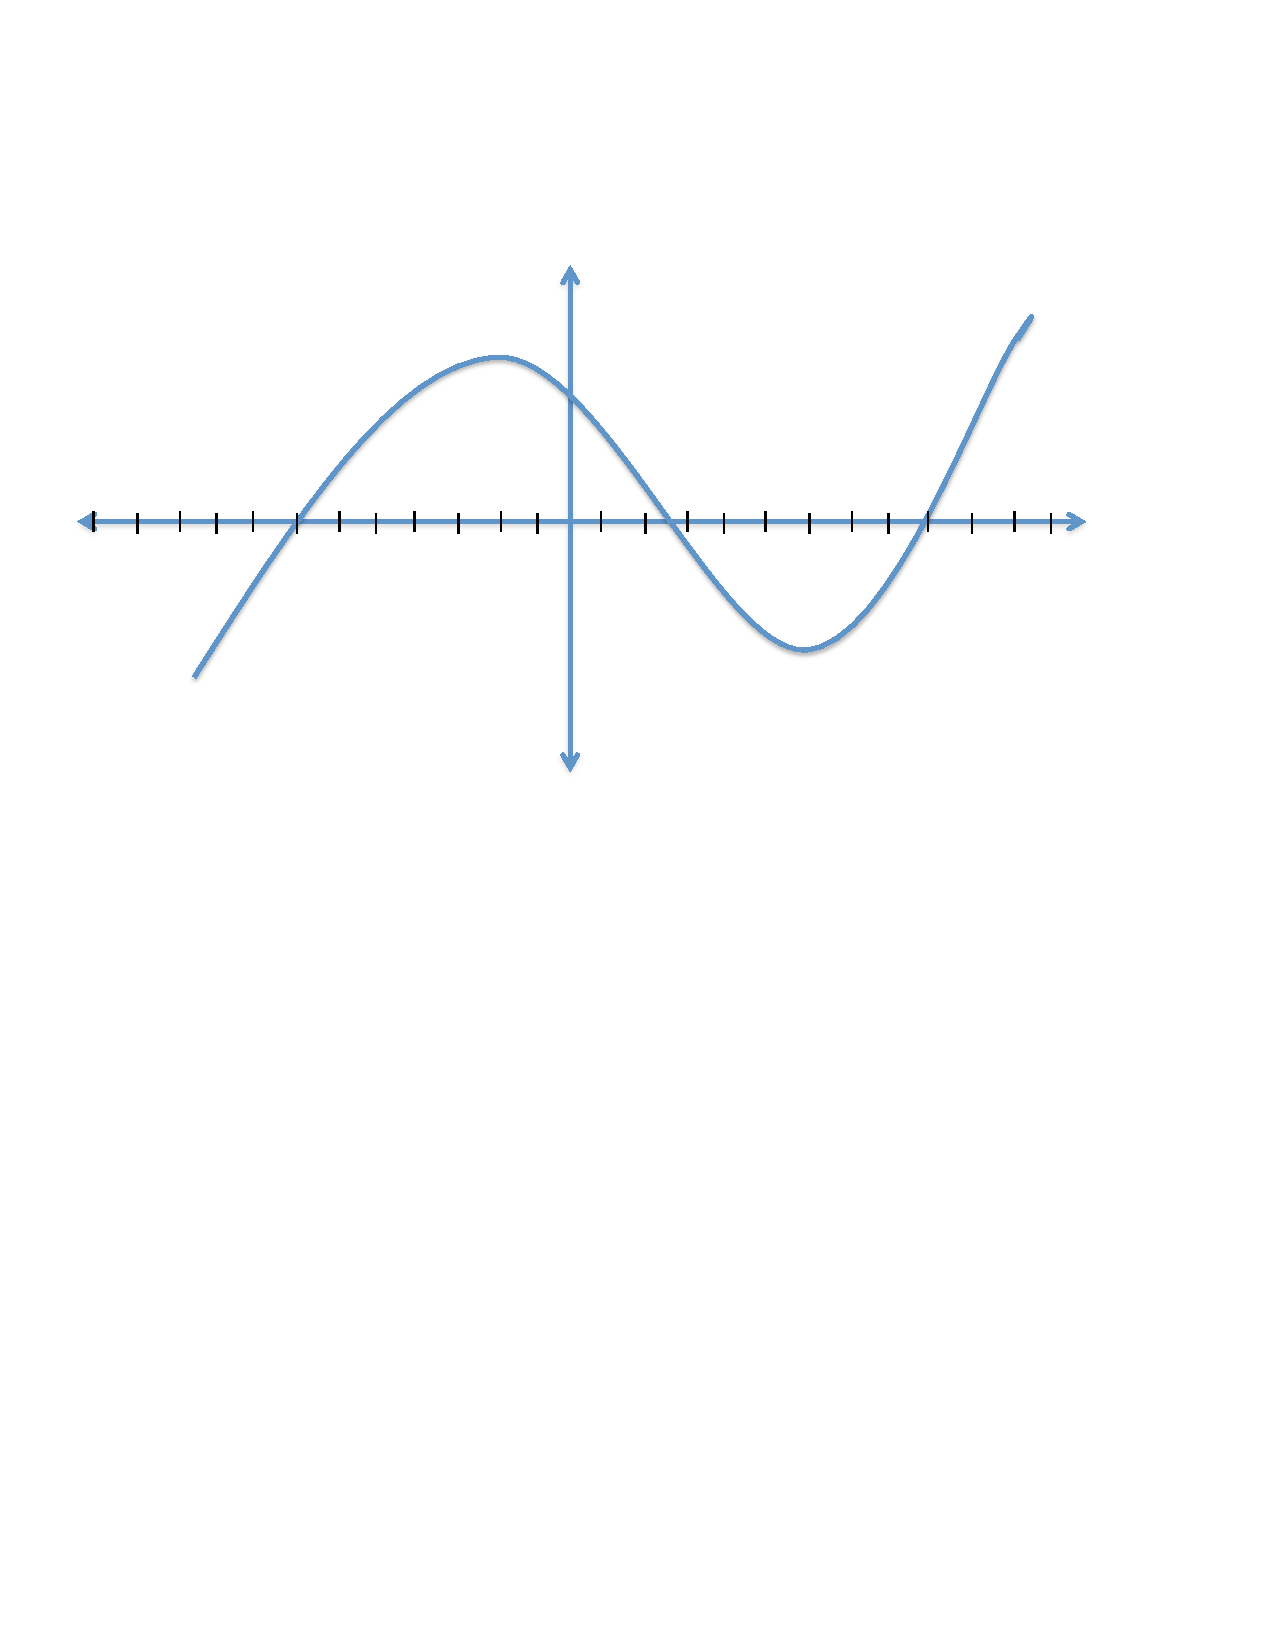
\includegraphics[trim= 140 420 290 180]{Images/Figure2.pdf}
	\end{image}
	
	\begin{enumerate}
	
	%part a
	\item  Describe the motion of the object as precisely as you can.
		\begin{freeResponse}
		Let us assume that $f(t)$ gives the position of John from his house at time $t$.  If $f(t) < 0$, then John is west of his house;  if $f(t) > 0$, then John is east of his house; if $f(t)=0$, then John is in front of his house.  
		
		For the first hour, that is, for $0 \leq t \leq 1$, John walks east away from his house.
		
		\begin{image}
		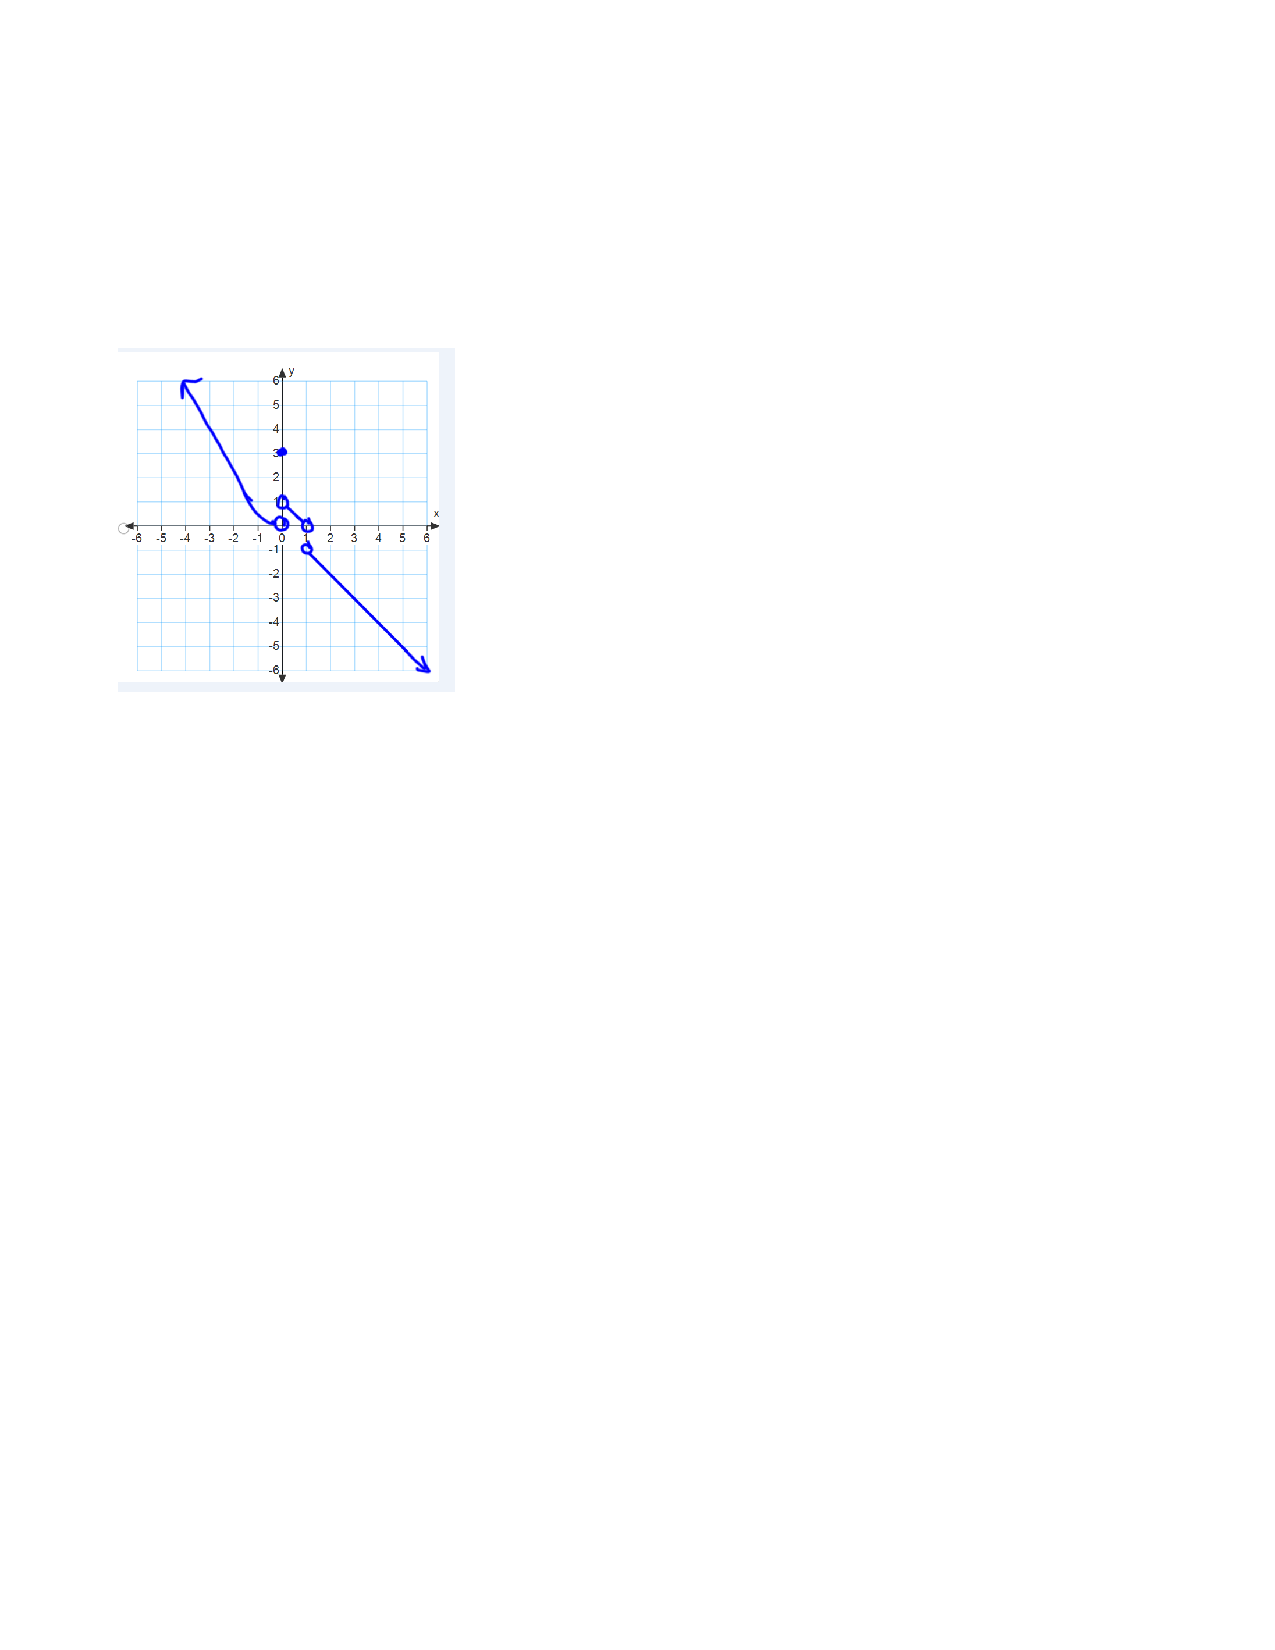
\includegraphics[trim= 140 570 290 200]{Images/Figure3.pdf}
		\end{image}
	
		For the second hour, that is, for $1 \leq t \leq 2$, John turns around and starts walking back west.  However, he does not walk all the way back to his house.
		
		\begin{image}
		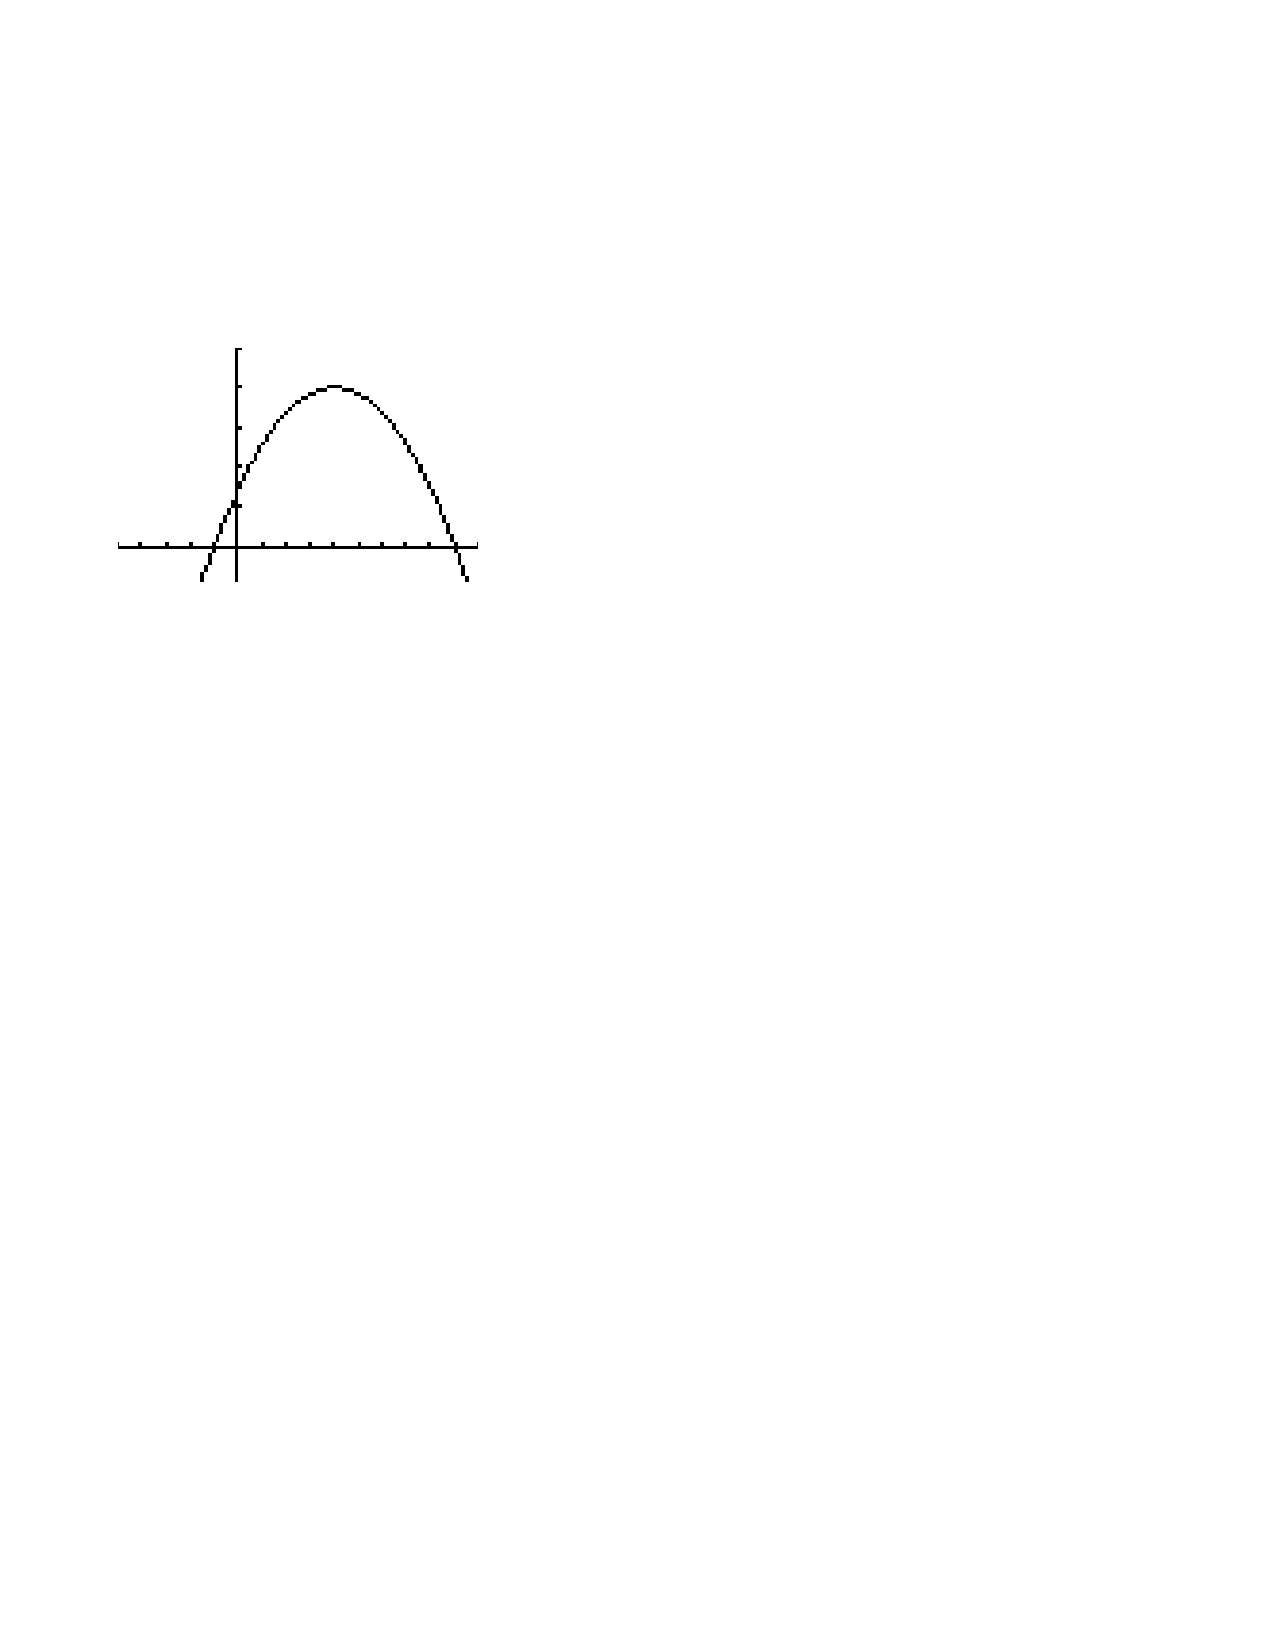
\includegraphics[trim= 140 570 290 200]{Images/Figure4.pdf}
		\end{image}
		
		For the third hour, that is, for $2\le t\le 3$, John realizes he needs to pick up an apple from the grocery store, which is way east of his house, for Elaine.  So he turns around again and walks east to the store.
		
		\begin{image}
		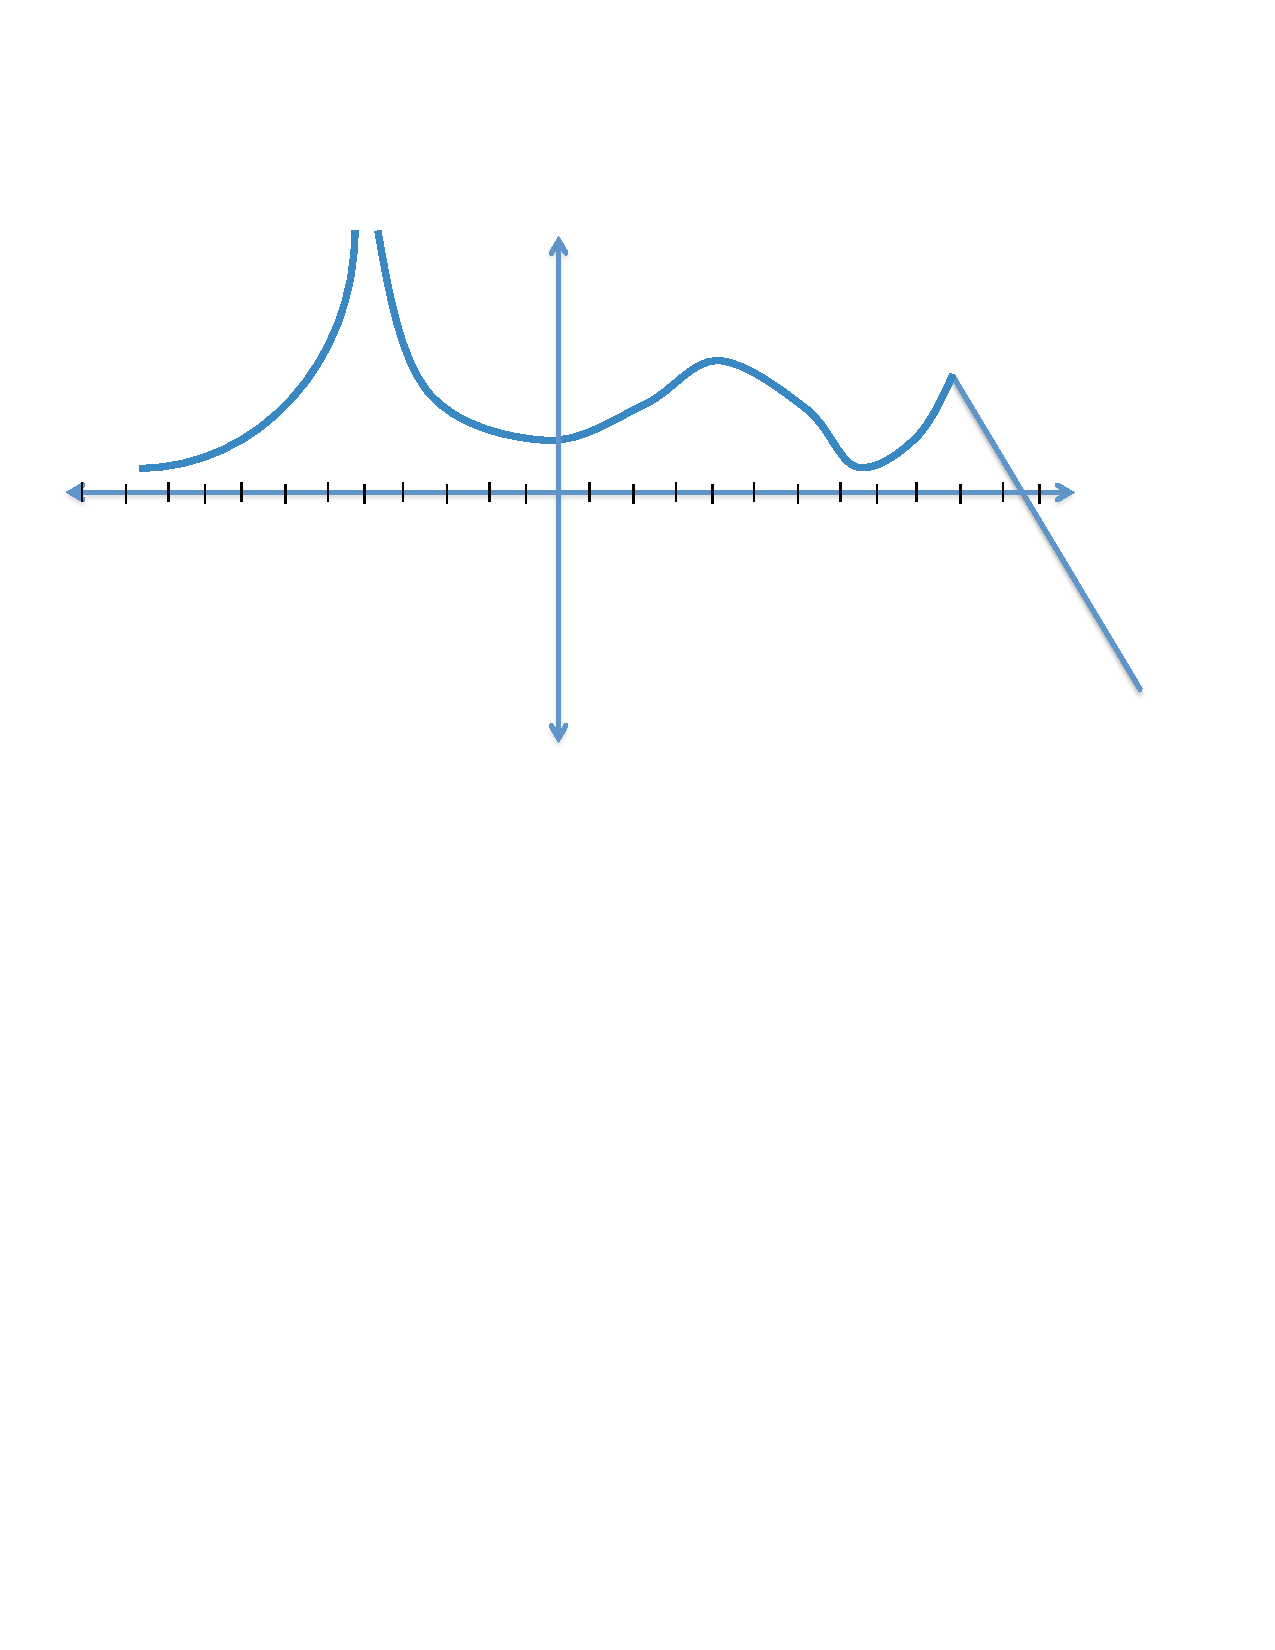
\includegraphics[trim= 140 570 290 200]{Images/Figure5.pdf}
		\end{image}
		
		For the fourth hour, that is, for $t \ge 3$, John needs to drop the apple off at Elaine's house, which is west of his house.  He turns west and walks past his house until he makes it to Elaine's house.
		
		\begin{image}
		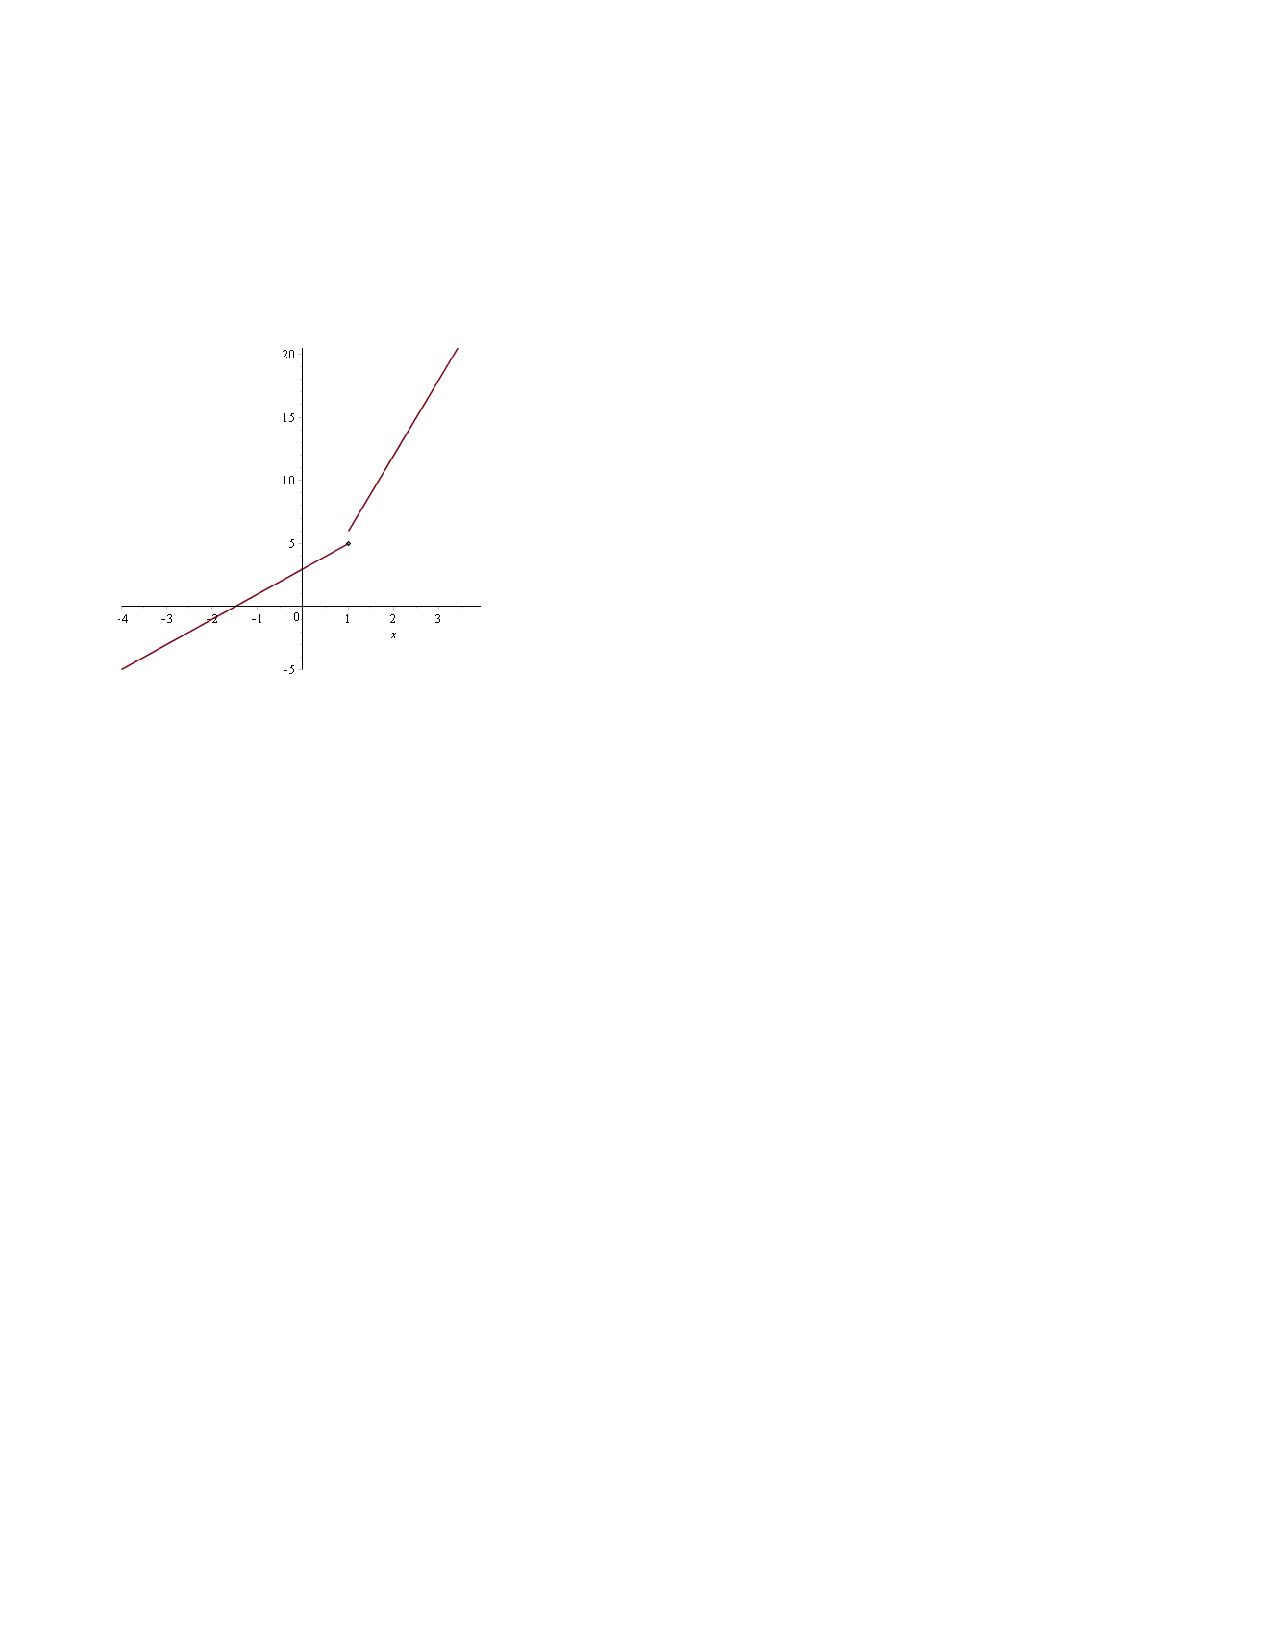
\includegraphics[trim= 140 540 290 200]{Images/Figure6.pdf}
		\end{image}

		\end{freeResponse}
		
	%part b
	\item  When is the velocity of the object zero?  What is happening to the object at those times? 
		\begin{freeResponse}
		John's velocity is zero at times $t=0,t=1,t=2$, and $t=3$ (the times where the slopes of the tangent lines are zero).  At these times, John changes direction since the slopes of the tangent lines to the graph of $f(t)$ change from positive to negative.
		\end{freeResponse}
		
	%part c
	\item  When is the object moving in the positive direction?  When is the object the furthest in the positive direction and the furthest in the negative direction?
		\begin{freeResponse}
		John is moving in the positive direction (in this story, east) during times in the region $(0,1) \cup (2,3)$.  John is furthest in the positive direction at time $t=3$ and furthest in the negative direction at (approximately) time $t=3.5$.
		\end{freeResponse}
		
	%part d
	\item  When is the object speeding up and slowing down? When is the object going at maximum velocity?
		\begin{freeResponse}
		John is speeding up in the region $(0,0.5) \cup (1, 1.5) \cup (2, 2.5) \cup (3, 3.5)$.  He is slowing down in the region $(0.5, 1) \cup (1.5, 2) \cup (2.5, 3)$.  John is moving the fastest at time $t = 3.5$, but that maximizes his speed, not his velocity, because he is moving in the negative direction at that time.  It appears that he maximizes his velocity at about $t=2.5$.  
		\end{freeResponse}
	\end{enumerate}
\end{problem}



\section{Extra Problems for Personal Practice}
          \begin{problem}
            \outcome{Recognize a composition of functions.}
            True or False: The function $e^{7x^2}$ can be differentiated without
            using the Chain Rule.
            \begin{freeResponse}
              False.
              $\ddx \left( e^{7x^2} \right) = e^{7x^2} \cdot \ddx
              \left( 7x^2 \right) = 14x e^{7x^2}$.
            \end{freeResponse}
          \end{problem}

\begin{problem}
    True or False: The derivative of a product is not the product of the derivatives.  But the derivative of a composition is a product of derivatives.
		\begin{freeResponse}
		True!
		
		$\ddx (f(x) g(x)) = f'(x) g(x) + f(x) g'(x)$.
		
		$\ddx(f(g(x))) = f'(g(x)) \cdot g'(x)$.
		\end{freeResponse}	
\end{problem}

\begin{problem}
  \outcome{Assign meaning to the first and second derivatives of a position function.}
  \outcome{Find velocity and acceleration and use them to determine information about position.}
  \mbox{}
  \begin{enumerate}
    % part a
    \item
      True or False:  If the acceleration of an object is constant, then its velocity is constant.
	
	%part b	
	\item  True or False:  A moving object can have negative acceleration and increasing speed.

	\end{enumerate}
\end{problem}

\begin{problem}
  \outcome{Assign meaning to the first and second derivatives of a position function.}
  \outcome{Find velocity and acceleration and use them to determine information about position.}
Suppose that a stone is thrown vertically upward from a cliff on Mars with an initial velocity of $64$ ft/s from a height of $192$ ft.  The height $s$ of the stone above the ground after $t$ seconds is given by $s(t) = -6t^2 + 24t + 192$.

	\begin{enumerate}
	
	%part a
	\item  Determine the velocity and acceleration of the stone after $t$ seconds.
			\begin{freeResponse}
			The velocity $v(t)$ is:  $v(t) = s'(t) = -12t + 24$.
			
			The acceleration $a(t)$ is:  $a(t) = v'(t) = s''(t) = -12$.
			\end{freeResponse}
			
			
			
	%part b
	\item  What is the greatest height of the stone and when does it occur?  What are the velocity and acceleration at that time?
			\begin{freeResponse}
			Since the function $s(t)$ is differentiable everywhere (it is a polynomial), the maximum height must occur at a time when the velocity is $0$.  So we solve:
			\begin{align*}
			v(t) = -12t+24 &:= 0 \\
			12t &= 24 \\
			t &= 2
			\end{align*}
			
			It is easy to check that $v(t) > 0$ for $0 \leq t < 2$ and $v(t) < 0$ for $2 < t$, and so the greatest height of the stone really does occur at time $t=2$.  The greatest height is $s(2) = -24 + 48 + 192 = 216$ ft.  For the second question we have already seen that $v(2) = 0$ ft/sec, and we have a constant acceleration of $-12$ ft/sec$^2$.  So $a(2) = -12$ ft/sec$^2$.
			\end{freeResponse}
			
			
			
	%part c
	\item  When does the stone hit the ground?  What are the velocity and acceleration at that time?
			\begin{freeResponse}
			The stone hits the ground when $s(t) = 0$.  So we solve:
			\begin{align*}
			s(t) = -6t^2 + 24t + 192 &:= 0 \\
			-6(t^2 - 4t - 32) &= 0 \\
			-6(t-8)(t+4) &= 0 
			\end{align*}
			
			Since we are only considering $t \geq 0$, we must have $t=8$.  At this instant, $v(8) = -96 + 24 = -72$ ft/sec and $a(8) = -12$ ft/sec$^2$.  
			\end{freeResponse}
				
	\end{enumerate}
\end{problem}

\end{document} 
